\documentclass[12pt,a4paper]{report}

\usepackage[top=1in, bottom=1in, left=1.25in, right=1.25in]{geometry}
\usepackage{graphicx}
\usepackage{float}
\usepackage{xeCJK}
% \usepackage{ctex}
\usepackage{algorithm}
\usepackage{algorithmicx}
\usepackage{algpseudocode}
\usepackage{listings}
\usepackage{color}
\usepackage{tikz}
\usepackage{fancyhdr}
\usepackage{amsmath,amssymb,amsthm}
\usepackage[toc,page]{appendix}
\usepackage{multirow}
\usepackage[utf8]{inputenc}
\usepackage{booktabs}
\usepackage[hidelinks]{hyperref}

\DeclareMathOperator*{\argmax}{arg\,max}

\definecolor{codegreen}{rgb}{0,0.6,0}
\definecolor{codegray}{rgb}{0.5,0.5,0.5}
\definecolor{codepurple}{rgb}{0.58,0,0.82}
\definecolor{backcolour}{rgb}{0.95,0.95,0.92}

\lstset{
	language=Python,
    backgroundcolor=\color{backcolour},   
    commentstyle=\color{codegreen},
    keywordstyle=\color{magenta},
    numberstyle=\tiny\color{codegray},
    stringstyle=\color{codepurple},
    basicstyle=\ttfamily\footnotesize,
    breakatwhitespace=false,         
    breaklines=true,                 
    captionpos=b,                    
    keepspaces=true,                 
    numbers=left,                    
    numbersep=5pt,                  
    showspaces=false,                
    showstringspaces=false,
    showtabs=false,                  
    tabsize=2,
	columns=flexible
}

\pagestyle{fancy}
\lhead{\leftmark}
\rhead{\reportTitle}
\renewcommand{\headrulewidth}{0.5pt}

\def\@maketitle{%
	\newpage
	\null
	\vskip 2em%
	\begin{center}%
	\let \footnote \thanks
    {\LARGE \@title \par}%
    \vskip 1.5em%
    {\large
    	\lineskip .5em%
    	\begin{tabular}[t]{c}% <------
        	\@author%          <------ Authors
      	\end{tabular}\par}%    <------
    \vskip 1em%
    {\large \@date}%
  	\end{center}%
  	\par
  	\vskip 1.5em}

\title{
	
\includegraphics[scale=0.7]{img/nycu_name.png}\\
	
\includegraphics[scale=0.5]{img/nycu_logo.pdf}\\
	~\\
	\LARGE\textbf{\reportSubtitle}\\
	\huge\textbf{\reportTitle}\\
}
\author{
	\begin{tabular}{rl}
		\textbf{Name: } & \authorName \\
		\textbf{Student ID: } & \authorStudentID  \\
	\end{tabular} \\~\\
	\authorDepartment
}

\newcommand{\reportTitle}{Programming Assignment \#1}
\newcommand{\reportSubtitle}{Image Processing}
\newcommand{\authorName}{許子駿}
\newcommand{\authorStudentID}{311551166}
\newcommand{\authorSchool}{National Yang Ming Chiao Tung University}
\newcommand{\authorDepartment}{Institute of Computer Science and Engineering}

\begin{document}
	\maketitle
	\tableofcontents
	\chapter{Description}
\indent\indent
	\textbf{Optical Character Reader (OCR)} is a useful tool. In this project, an OCR to recognize music notes is implemented. \\
	If a stave is input to be recognize, first, locate the five horizontal lines and capture the region. Second, extract the music notes from the captured image. 
	Third, input the extracted music notes to the Convolutional Neural Network (CNN) model; then, the model will recognize each music note. \\
	In this project, the most important part, the third part, is implemented. \\
	For the selected data set, the accuracy rate can be \textbf{98\%}.


%	\chapter{Algorithm specification}
\indent\indent
	In this project, a simple CNN model is implemented to recognize music notes. \\
	

	\chapter{Analysis and comments}
\indent\indent
	In this project, a simple CNN model is implemented to recognize music notes. \\
	This CNN model is developed by \textbf{Python3} and \textbf{Keras}.
	
%%
\section{Network structure}
\indent\indent
	Network structure:
	\begin{enumerate}
		\item \textbf{32} convolutional layers with $4 * 4$ kernel size.
		\item A \textbf{RELU} activation function.
		\item \textbf{1} max pooling layer with $2 * 2$ kernel size.
		\item Dropout with \textbf{25\%} probability to prevent from over-fitting.
		\item A \textbf{256}-dimensions fully connected (FC) layer.
		\item A \textbf{RELU} activation function.
		\item Dropout with \textbf{50\%} probability.
		\item A \textbf{9}-dimensions fully connected (FC) layer to classify.
		\item A \textbf{Softmax} layer.
	\end{enumerate}

	\begin{figure}[H]
		\centering
		\label{anal_1}
		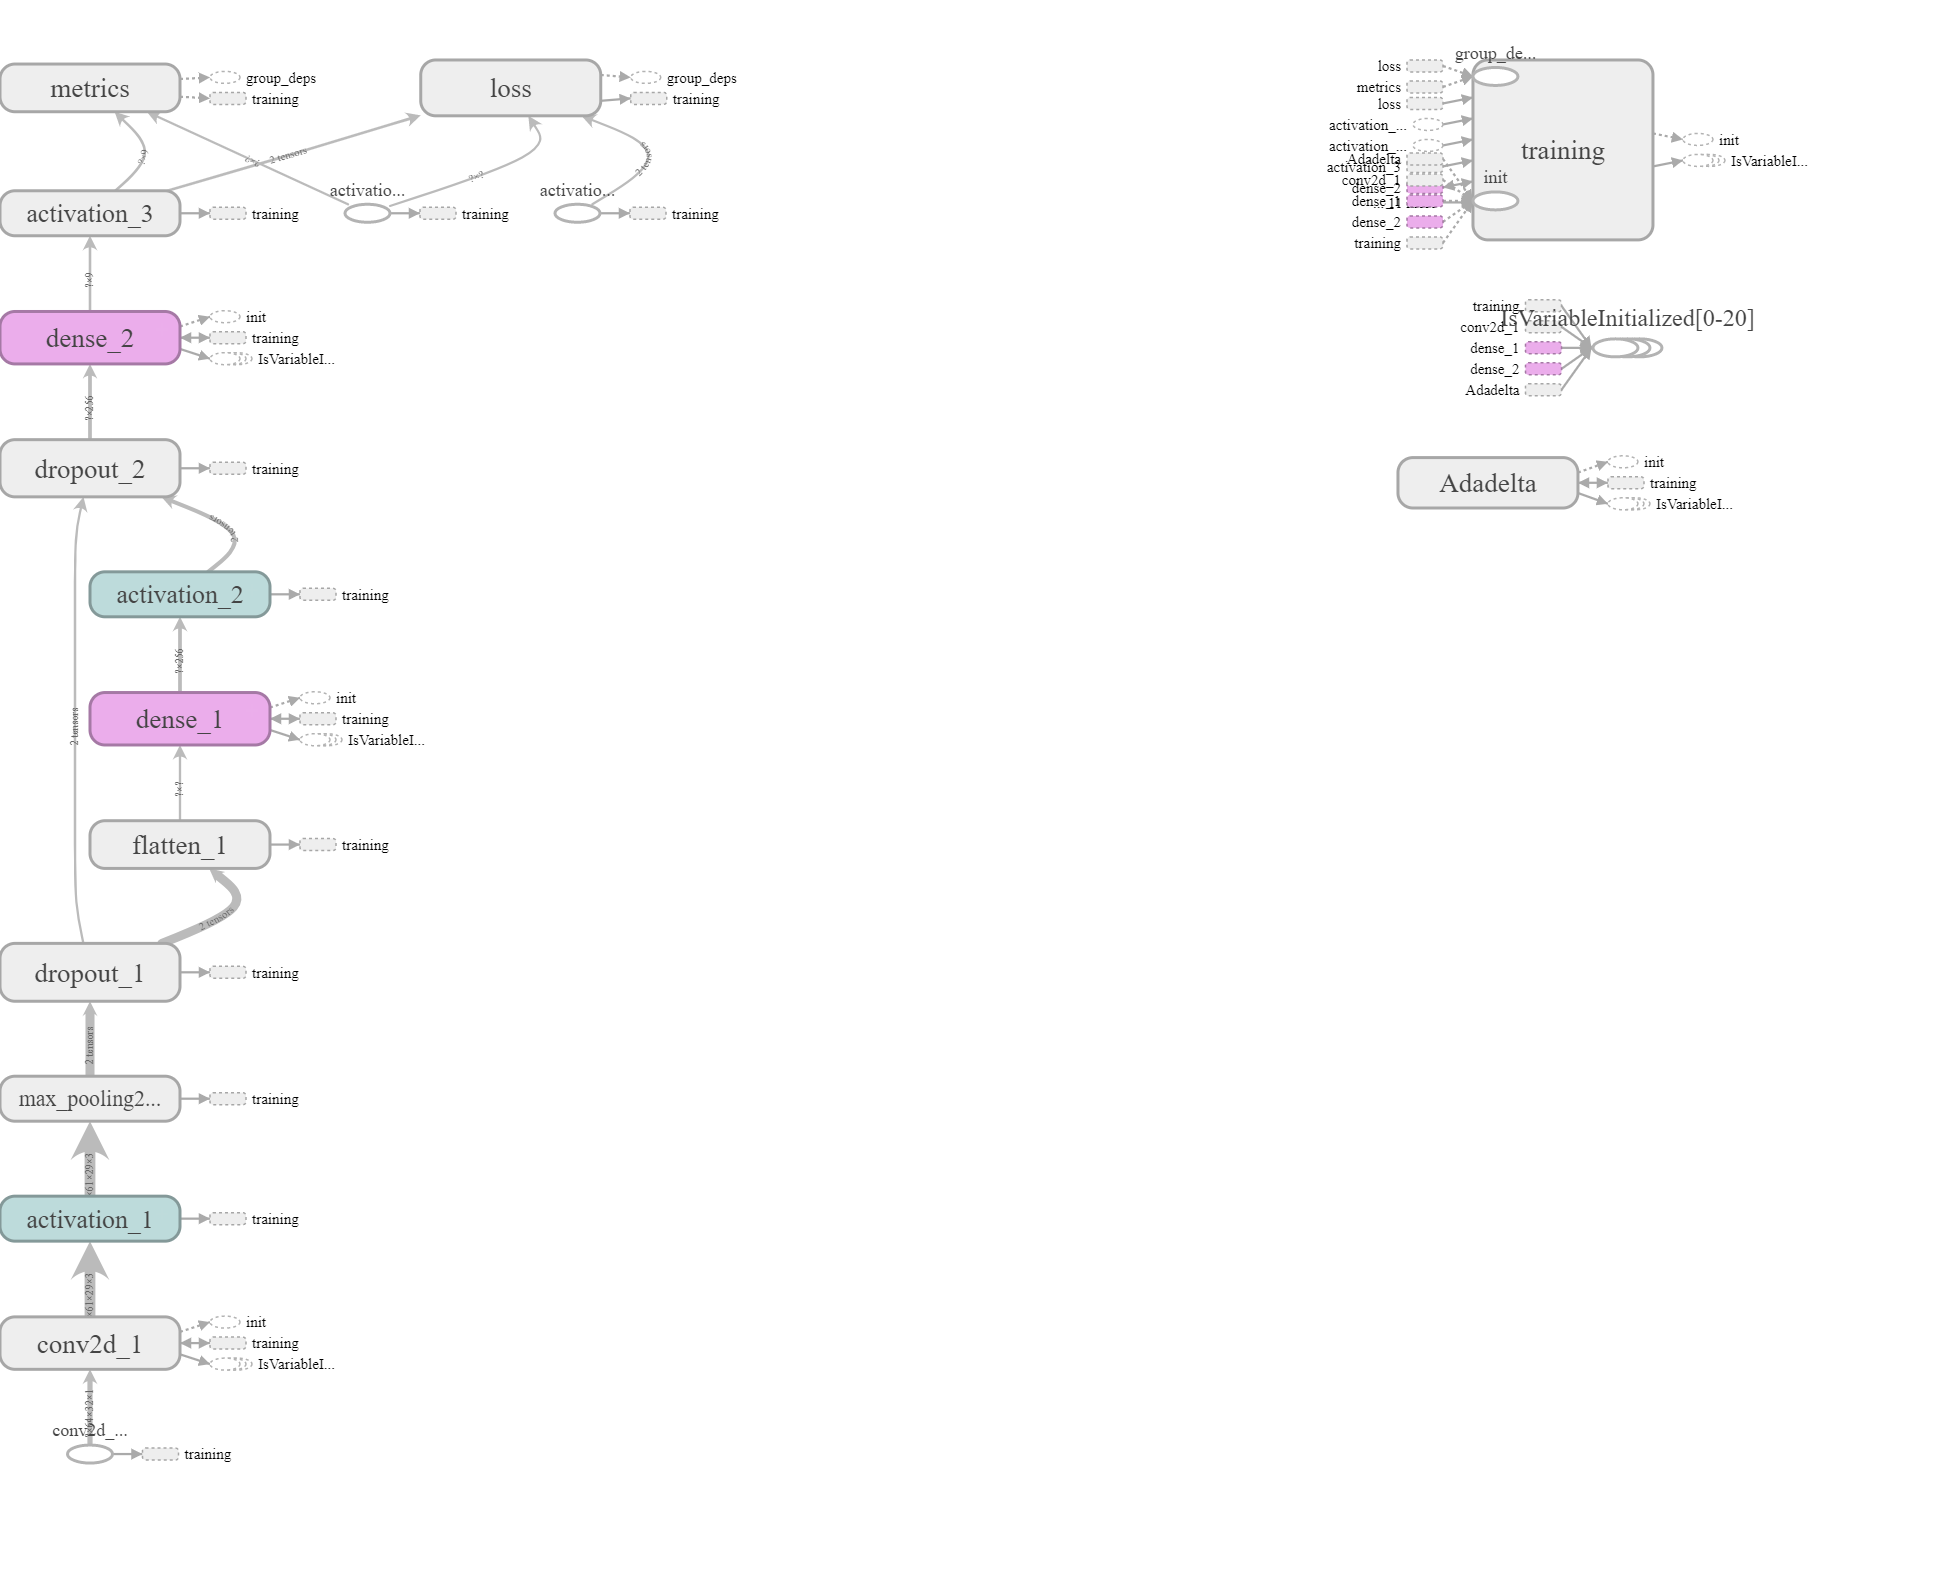
\includegraphics[scale=0.25]{img/sample_tensorboard.png}
		\caption{Tensorboard.}
	\end{figure}

%%
\section{Analysis}
\indent\indent
	In the figure \ref{anal_2}, the accuracy rate can be \textbf{98\%} in \textbf{8} epochs, and it shows the network structure works well for the testing data set.

	\begin{figure}[H]
		\centering
		\label{anal_2}
		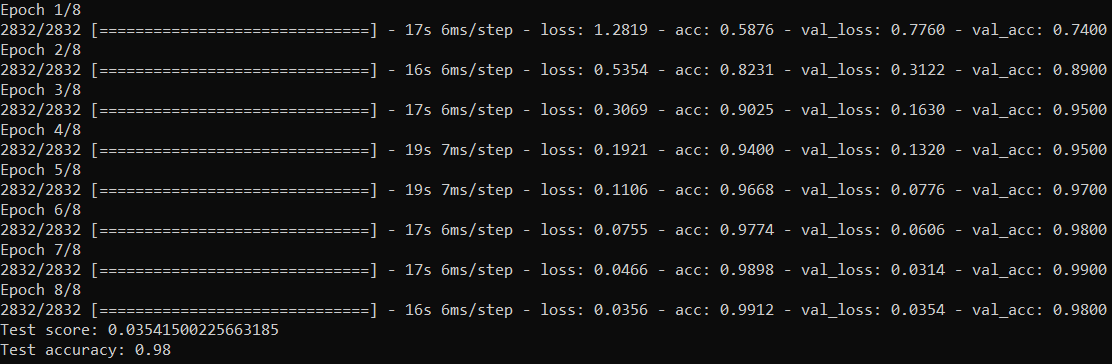
\includegraphics[scale=0.5]{img/sample_train_1.PNG}
		\caption{Accuracy rate.}
	\end{figure}
	


	\chapter{Conclusion}
\indent\indent
	The network structure for CNN is a problem, I have tried several times to make the network works better. \\
	However, The network structure maybe work well only for this data set. 
	If the network structure is not well-selected and the data set is too small, it may over-fit. \\
	OCR is a cool implementation using deep learning and usually seen in normal life. It can be also used for another object and the result will be significant, 
	and make lives more convenient.
	

	\begin{appendices}
		\chapter{Code}
\lstinputlisting[caption=music\_note\_ocr.py]{code/music_note_ocr.py}

	\end{appendices}
\end{document}
